\documentclass[]{article}

\title{User's Manual for Genair}
\author{Hugo Gagnon}
\date{February 1, 2015}


\usepackage{graphicx}
\usepackage{rotating}
\usepackage{amsmath,amssymb}
\usepackage[para,multiple]{footmisc}
\usepackage[hyperfootnotes=false]{hyperref}


\setcounter{secnumdepth}{3}
\setcounter{tocdepth}{2}



\begin{document}



\maketitle
\tableofcontents


\newpage
\section{Preliminaries}

\subsection{Scope}
\label{subsec:scope}

Genair is a high-fidelity conceptual aircraft design tool.  At the 
moment it is most useful to generate the outer mold line of general 
aircraft such as the blended wing-body, the box wing, the truss-braced 
wing, etc.  It does that through a component-based approach, whereby 
wings, fuselages, nacelles, etc., can be arbitrarily assembled in 
three-dimensional space.

Genair has been developed for high-fidelity, exploratory aerodynamic 
shape optimization.  As such, it emphasizes on \emph{high-quality} 
surfaces, \emph{flexible} aircraft components, and an \emph{interactive} 
interface.  The graphical capability of the interface has been kept to a 
minimum.  The intention was to prioritize the development of an 
intuitive API meant to steer large-scale, multidisciplinary 
optimizations.

Genair parameterizes aircraft components with non-uniform rational 
B-spli\-nes~(NURBS), the same mathematical representation used in CAD.  
Hence, Genair can be thought of as a hybrid between CAD and a parametric 
aircraft design tool.  The main difference with CAD is that model 
topology is ignored.  Moreover, surface trimming at wing-body junctions 
and the like is still somewhat experimental.\footnote{In practice, at 
least in Prof.\ David Zingg's research group, these limitations are 
inconsequential since, first, we assume fixed topology throughout an 
optimization, and, second, surface trimming is in any case best handled 
by the geometry kernel (e.g.\ Parasolid) native to the mesh generator 
(e.g.\ ANSYS ICEM CFD) used to generate a watertight grid.}

Genair uses object-oriented programming in Python to encapsulate 
aircraft components.  Each component defines its own ``construction 
recipe'', thereby hiding most of the geometry generation process to the 
user.  Naturally, a good understanding of NURBS or even Python is still 
required when designing custom shapes or implementing new components.

\subsection{Suggested Readings}

Genair is not your typical CAD package, in that it remains a fairly 
low-level library of classes and functions.  The advantage is an 
increase in flexibility; the disadvantage is the steep learning curve.

Here are some topics I suggest you brush up on before you install 
Genair.

\subsubsection{Non-Uniform Rational B-Splines}

Anyone serious about aircraft design should know about NURBS.  The go-to 
reference for NURBS is, surprise surprise, ``The NURBS 
Book''~\cite{Piegl1997}.  I suggest you read Chapters~1 to 4, and skim 
through Chapters~5 to 10.  If you are short on time then at least read 
``On NURBS: a survey''~\cite{Piegl1991}.

By the end of your readings you should be able to answer questions such 
as: what is the effect of multiple knots or coincident control points on 
the geometric and parametric continuity of NURBS curves and surfaces?

\subsubsection{Free-Form Deformation}

Free-form deformation~(FFD)~\cite{Sederberg1986} is not only central to 
the geometry control system implemented in Jetstream 
(Appendix~\ref{app:jetstream}), but is also used in Genair for the 
manual design of aircraft components.  In both cases a significant 
departure from standard FFD is the fact that it is the control points of 
the deforming objects that are manipulated as opposed to their 
discretization.

\subsubsection{Python, NumPy, and IPython}

To use Genair effectively you will need a working knowledge of Python.  
Fortunately, Python is very easy to learn and use.  I suggest you read 
``The Python Tutorial'', which is part of the standard 
documentation~\cite{python}.  Pay special attention to the chapters on 
``Data Structures'' and ``Classes''.

What makes Python a scientific computing language comparable to Matlab 
is NumPy.  Genair makes extensive use of NumPy's ``array object''.  To 
learn about the array object and its use in linear algebra I suggest you 
read the ``Tentative NumPy Tutorial''~\cite{numpy}.  Pay special 
attention to the section on ``Copies and Views''.

Finally, Genair uses IPython for its command-line interface.  IPython 
can be thought of as the ``Command Window'' of Matlab but for Python.  I 
suggest you read the ``Introduction'' chapter of IPython's 
documentation~\cite{ipython}.  Pay special attention to the section 
called ``Enhanced interactive Python shell'', including the subsection 
called ``Main features of the interactive shell''.


\section{Introduction}

\subsection{Installation}

\subsubsection{Python Distribution}
\label{subsubsec:anaconda}

Before you install Genair you will need a Python 2 
interpreter~\cite{python} along with the NumPy~\cite{numpy}, 
SciPy~\cite{scipy}, IPython~\cite{ipython}, PyOpenGL~\cite{pyopengl}, 
pyglet~\cite{pyglet}, and PIL~\cite{pil} packages.  While it is possible 
to install all of these using the standard Distutils, I highly recommend 
using a third-party Python distribution such as Continuum Analytics' 
Anaconda~\cite{anaconda}.  Anaconda is free of charge and ships with a 
very handy package manager called ``conda''.

The following instructions assume that you have installed Anaconda, but 
they can be easily adapted to any Python distribution.

If you have not already done so, start by updating conda followed by 
Anaconda itself:
\begin{verbatim}
$ conda update conda
$ conda update anaconda
\end{verbatim}
Next, create a new conda environment called ``genair'' and activate it 
in your current shell:
\begin{verbatim}
$ conda create -n genair pip
$ source activate genair
\end{verbatim}
The second command should have modified your shell path and prepended 
the string ``\texttt{(genair)}'' to your terminal prompt.  To install 
the packages listed above proceed with
\begin{verbatim}
(genair)$ conda install ipython numpy scipy pil
\end{verbatim}
Then, depending on whether ``\texttt{conda search pyopengl}'' returns 
something or not (as of February 2015 it does on OS X but not on Linux), 
use either one of
\begin{verbatim}
(genair)$ conda install pyopengl
\end{verbatim}
or
\begin{verbatim}
(genair)$ pip install pyopengl
\end{verbatim}
Finally, install pyglet:
\begin{verbatim}
(genair)$ pip install pyglet
\end{verbatim}

To test IPython and NumPy, try the following in a new terminal:
\begin{verbatim}
(genair)$ ipython
\end{verbatim}
which should put you in an IPython shell.  From there type\footnote{By 
convention, in this manual the default Python prompt (\texttt{>>>}) is 
used rather than IPython's prompt (\texttt{In [n]}, where $n \in 
\mathbb{Z}^+$).}
\begin{verbatim}
>>> import numpy as np
>>> np.__version__
\end{verbatim}
and see if the version string matches the one returned by 
``\texttt{!conda list}''.

From time to time, say every other month, you may want to update the 
packages to their latest version:\footnote{Repeat the second command for 
PyOpenGL if you installed it with pip.}
\begin{verbatim}
(genair)$ conda update --all
(genair)$ pip install --upgrade pyglet
\end{verbatim}

\subsubsection{Genair}

Installing Genair should be as simple as
\begin{verbatim}
$ git clone /nfs/carv/d1/people/comp-aero/genair.git
\end{verbatim}
To test your clone of Genair, ``\texttt{cd}'' into ``\texttt{genair/}'' 
and type\footnote{The first command assumes that you are using Anaconda; 
see the previous section.}
\begin{verbatim}
$ source activate genair
(genair)$ ./main.py
\end{verbatim}
which should, again, put you in an IPython shell.  The real test, 
however, is whether pyglet supports your graphics card.  If it does 
\emph{not} then you probably already know it from the error messages 
triggered by executing ``\texttt{main.py}''.  If there were no such 
messages then cross your fingers and try this one last command:
\begin{verbatim}
>>> draw(Point())
\end{verbatim}
which should open a black window with a yellow point in the middle of 
it.  You can close that window by pressing the Escape key and you can 
exit Genair like you would exit IPython, i.e.\ by typing 
``\texttt{exit}'' at the prompt.

\subsection{Quick Start}
\label{subsec:quick}

To give you a sense of what Genair can do I propose to go over a simple 
tutorial where you will generate a box wing.

Start by launching Genair:\footnote{Again, the first command assumes 
that you are using the Anaconda Python distribution; see 
Section~\ref{subsubsec:anaconda}.}
\begin{verbatim}
$ source activate genair
(genair)$ ./main.py
\end{verbatim}
which will automatically put you in the ``\texttt{play/}'' subdirectory 
of Genair's root directory.\footnote{The ``\texttt{play/}'' subdirectory 
is not tracked by Git so use it as you please.}  You can see this for 
yourself by typing ``\texttt{\%pwd}'' at the prompt.\footnote{In 
IPython, the ``\texttt{\%}'' character denotes a magic function.  To 
learn more about IPython's magic function system type 
``\texttt{\%magic}''.}  By typing ``\texttt{\%ls}'' you will also see 
that there is an ``\texttt{airfoils/}'' directory in ``\texttt{play/}''.  
``\texttt{\%cd}'' into it and type ``\texttt{\%ls}'' once again.  As you 
can see the directory already contains a number of airfoil data files.

For this first tutorial you will fit the NACA 0012 airfoil.  To do so 
you will need the Airfoil class, but first you should learn how to use 
it.  In Genair, the easiest way to get information is through the 
``\texttt{?}'' operator, e.g.\footnote{The ``\texttt{?}'' operator is 
another extremely useful feature of IPython; it lets you inspect an 
object's docstring without leaving the prompt.  Similarly, the 
``\texttt{??}'' operator lets you inspect not only an object's docstring 
but also its source code.  Both ``\texttt{?}'' and ``\texttt{??}'' can 
be used on \emph{any} Python object, e.g.\ try using them on the 
``\texttt{\%pwd}'' magic function.}
\begin{verbatim}
>>> Airfoil?
\end{verbatim}
Notice how the docstring tells you what the Airfoil class does and in 
particular how it is intended to be used.  In this case, it just so 
happens that the example given also uses the NACA 0012 airfoil, so go 
ahead and follow it step by step, starting with:
\begin{verbatim}
>>> af = Airfoil(`n0012.dat')
\end{verbatim}
This commands creates an instance of the Airfoil class and assigns it to 
the variable ``\texttt{af}''.\footnote{At this point it is worth 
mentioning that, similar to Matlab, IPython can list the variables 
defined in your namespace by typing ``\texttt{\%whos}''.}

The output of the previous command will have informed you that the data 
file contains 132 points.  Indeed, for this particular instance of the 
NACA 0012 airfoil, the lower and upper halves are each defined with 66 
points.  Type ``\texttt{!head n0012.dat}'' to verify this information.  
Note also that the first line of ``\texttt{n0012.dat}'' has been stored 
in
\begin{verbatim}
>>> af.name
\end{verbatim}
In contrast, the ``\texttt{issymmetric}'' and ``\texttt{issharp}'' 
attributes are both evaluated at runtime.

At this point feel free to inspect the data points in an OpenGL 
window:\footnote{The reason why this command draws points and not a 
NURBS curve is because the airfoil has not beeen fitted yet.}
\begin{verbatim}
>>> draw(af)
\end{verbatim}
Press the F2 key to switch to a $xz$ view and then zoom in using the 
mouse middle button.\footnote{The OpenGL interface is explained in 
Section~\ref{subsec:opengl}.  Meanwhile, have a look at the header of 
``\texttt{plot/controller.py}''.}  When you are done close the window by 
pressing the Escape key.\footnote{As explained in 
Section~\ref{subsec:opengl}, although Genair supports multiple windows 
running at the same time, it is best to close them when not needed.}

Next, proceed with the remaining instructions of the 
example:\footnote{Don't forget to use the ``\texttt{?}'' operator to 
learn about the purpose and default arguments of each method.}
\begin{verbatim}
>>> af.fit()
>>> af.sharpen()
>>> af.fit()
>>> af.transform()
\end{verbatim}
The last method transforms the airfoil so that its chord length becomes 
unity and its quarter-chord point coincides with the global 
origin.\footnote{These transformations matter when constructing a Wing 
object (Section~\ref{subsubsec:wing}).}

You should now save your work to avoid repeating the same steps 
everytime you want to use a NACA 0012 airfoil.  Start by making a new 
subdirectory in ``\texttt{play/}'' called ``\texttt{tutorial/}'', 
``\texttt{\%cd}'' into it, and then save your Airfoil object 
likewise:\footnote{Try the ``\texttt{\%mkdir} magic 
function.}\footnote{The next section gives an overview of the saving and 
loading mechanism.}
\begin{verbatim}
>>> save(af, fn=`n0012.p')
\end{verbatim}
For the sake of demonstration, relaunch Genair, navigate to 
``\texttt{tutorial/}'', and type
\begin{verbatim}
>>> af, = load(`n0012.p')
\end{verbatim}
The Airfoil object that ``\texttt{af}'' now points to should be in the 
same exact state than before and can thus be used in the same exact way.

Now to the box wing.  We will assume that the three wing segments 
(lower, tip fin, and upper) meet at right angles.\footnote{An 
alternative would be to generate smooth corner fillets.}  This time you 
will need the Wing class, so, as before, start by learning about it:
\begin{verbatim}
>>> Wing?
\end{verbatim}
Unsurprisingly, the docstring informs you that you need at least one 
Airfoil object to instantiate a Wing object.  So go ahead and type
\begin{verbatim}
>>> lower = Wing(af)
\end{verbatim}
Next, create the ``trajectory curve'' along which ``\texttt{af}'' will 
be swept:\footnote{This is a common example of where you are required to 
directly interact with the NURBS library.  The library is discussed in 
Chapter~\ref{cha:nurbs}; for now, to see other functions available in 
its ``toolbox'', type ``\texttt{nurbs.tb.}''\ at the prompt followed by 
the Tab key.}
\begin{verbatim}
>>> T = nurbs.tb.make_linear_curve(Point(), Point(y=3))
\end{verbatim}
Assuming that you don't want any twist nor any taper you can finalize 
the Wing object with the following two commands:\footnote{As explained 
in Section~\ref{subsubsec:wing}, twist and taper are easily specified 
through B-spline functions.}\footnote{By default, the second command 
will show you the NURBS representation of the final Wing object.  In 
Genair, keep in mind that what you see is only a \emph{triangulation} of 
the actual NURBS curves and surfaces.  Type ``\texttt{draw?}'' to find 
out more.}
\begin{verbatim}
>>> lower.orient(T)
>>> lower.fit()
\end{verbatim}
Finally, give it some sweep:\footnote{Alternatively, one could have 
generated a trajectory curve with the point 
``\texttt{Point(x=1.73205081, y=3, z=0)}'' before orienting and fitting 
the wing.  Try it!}\footnote{The ``glue/unglue'' mechanism is explained 
in Section~\ref{subsubsec:methods}.  Basically, it is necessary so that, 
for example, when sweeping a wing not only does its NURBS representation 
shear but also its trajectory curve, wing tip (if any), etc.}
\begin{verbatim}
>>> lower.glue()
>>> lower.sweep = 30
\end{verbatim}
To generate the tip ``\texttt{fin}'' Wing object, repeat the same exact 
process but use ``\texttt{Point(z=1)}'' instead of 
``\texttt{Point(y=3)}''.  Also, instead of sweeping it, give it a 90 
degree dihedral:
\begin{verbatim}
>>> fin.glue()
>>> fin.dihedral = 90
\end{verbatim}
You could use a similar approach to generate the ``\texttt{upper}'' Wing 
object, but in this case it is more convenient to simply copy the 
``\texttt{lower}'' Wing object and to give to that copy a 180 degree 
dihedral:\footnote{Again, this example reflects the fact that in Genair 
there are often multiple ways to arrive at the same result.}
\begin{verbatim}
>>> upper = lower.copy()
>>> upper.glue()
>>> upper.dihedral = 180
\end{verbatim}
Now is a good time to save your work:
\begin{verbatim}
>>> save(lower, fin, upper, fn=`lower_fin_upper.p')
\end{verbatim}

You may have noticed that all three wing segments are positioned 
relative to the global origin.  (See it for yourself: 
``\texttt{draw(lower, fin, upper)}''.)  What remains to be done is to 
connect them one after the other and to make sure that the connections 
are watertight.  The WingMerger class does that for you:
\begin{verbatim}
>>> box = WingMerger(lower, fin, upper)
>>> box.merge()
\end{verbatim}

Finally, you should save your work one last time:
\begin{verbatim}
>>> save(box, fn=`box.p')
\end{verbatim}
and perhaps even export the geometry in IGES format if you intend on 
using it in an external application such as ANSYS ICEM CFD.  The next 
section describes how to do this.

\subsection{Saving and Loading}
\label{subsec:ft}

The ``\texttt{save}'' and ``\texttt{load}'' functions demonstrated in 
the previous section are thin wrappers built around the 
``\texttt{cpickle}'' module.\footnote{Part of the Python's standard 
library~\cite{python}.}  A ``pickle'' is a binary file, typically with 
the extension ``\texttt{.p}'', that stores any number of any Python 
objects (well, almost).  In Genair, pickles are typically very small in 
size and are thus ideal to share work with others.

It is important to understand that pickles are not specific to Genair.  
For example, the snippet
\begin{verbatim}
>>> def power2(x):
...     return x**2
>>> save(0.1, np.array([3, 2, 1]), power2)
\end{verbatim}
works as expected.

You have probably figured out by now that the ``\texttt{save}'' function 
can take an arbitrary number of arguments.  Conversely, 
``\texttt{load}'' takes only one argument but returns a list of 
arbitrary length.  While intuitive, this approach works best if you are 
familiar with the concept of ``unpacking''.\footnote{This concept is 
also very useful when it comes to using the ``\texttt{draw}'' function 
described in Section~\ref{subsubsec:draw}.}  For example, assuming 
``\texttt{a}'' is a Python list of length 3, use
\begin{verbatim}
>>> save(*a)
\end{verbatim}
instead of
\begin{verbatim}
>>> save(a[0], a[1], a[2])
\end{verbatim}
Similarly, use
\begin{verbatim}
>>> a0, a1, a2 = load()
\end{verbatim}
instead of\footnote{The second command is more succintly written as: 
``\texttt{a0, a1, a2 = a}''.}\footnote{FYI length-1 sequences can also 
be unpacked, e.g.\ ``\texttt{a0, = a}'' versus ``\texttt{a0 = a[0]}''.}
\begin{verbatim}
>>> a = load()
>>> a0 = a[0]; a1 = a[1]; a2 = a[2]
\end{verbatim}

The ``\texttt{geom.io}'' module defines a few other functions related to 
I/O.\footnote{Again, use the tab completion feature of IPython to see 
all available functions.}  Out of those you will probably find 
``\texttt{save\_IGES}'' most useful.  Note that ultimately 
``\texttt{save\_IGES}'' only saves points and NURBS curves and surfaces; 
everything else gets discarded.  For example, assuming ``\texttt{af}'' 
is an Airfoil object, then
\begin{verbatim}
>>> geom.io.save_IGES(af)
\end{verbatim}
only saves the NURBS curves representing the lower and upper portions of 
the airfoil.\footnote{To be precise, its data points would be saved if 
the airfoil is not fitted.  This is because ``\texttt{save\_IGES}'' only 
saves what would be displayed by the ``\texttt{draw}'' function, i.e.\ 
what is returned by the ``\texttt{\_draw}'' method of a Part object.  
More on this topic in Sections~\ref{subsubsec:draw} and 
\ref{subsubsec:methods}.}

\subsection{Code Overview}

If you have read and understood Sections~\ref{subsec:quick} and 
\ref{subsec:ft} then you already know more about Genair than you think.  
To learn about some other useful features, e.g.\ geometrically nonlinear 
wings and automatically generated wingtips, you can go ahead and jump to 
the relevant sections without worrying too much about the code 
structure.

If, on the other hand, you plan on implementing new features, or even on 
becoming proficient with Genair, I strongly suggest that you spend some 
time understanding the machinery behind the interface.  Indeed, the true 
intent of this manual is not so much as documenting each and every 
aspect of Genair as to explaining its design philosophy.

\begin{sidewaysfigure}
  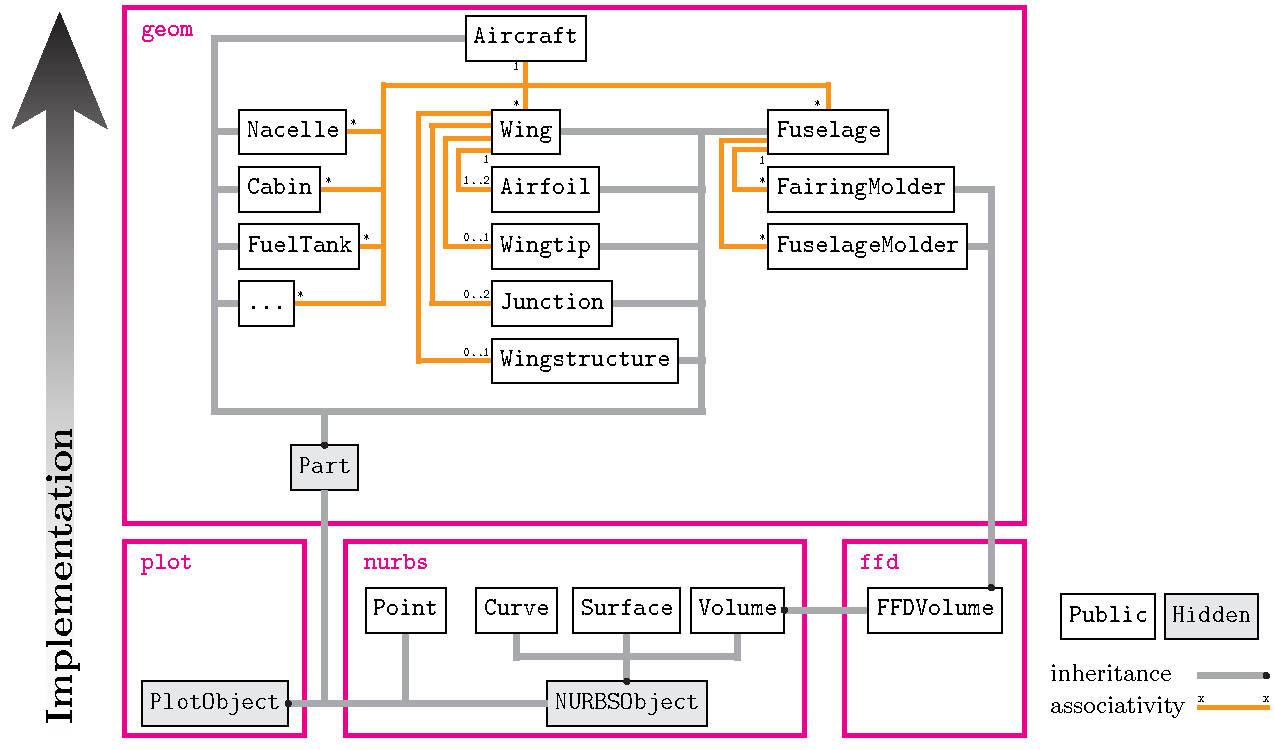
\includegraphics[width=\textwidth]{uml.pdf}
  \caption{%
Partial class diagram of Genair.  In the associativity tree, the symbol 
$\ast$ denotes ``zero or more instances'' and the notation $y..z$ 
denotes from ``$y$ to $z$ instances''.}
  \label{fig:uml}
\end{sidewaysfigure}

Central to this philosophy is the notion of inheritance.  As seen from 
the class diagram of Figure~\ref{fig:uml}, all classes defined in Genair 
(at least those shown here) are derived from the PlotObject class, which 
means that an instance of any one of those classes will be recognized by 
the ``\texttt{draw}'' function.  This is easily remembered.  In general, 
the end-user (you) only needs to know about three ``fundamental'' 
classes: Point, NURBSObject, and Part (all of which are shown in 
Figure~\ref{fig:uml}).  The first is universal and easily understood.  
The other two are specific to Genair and are based on the same general 
principle that a superclass inherits the properties and methods of its 
base class.  For example, the FFDVolume class inherits its 
``\texttt{.p}'' attribute from the NURBSObject class and the Wing class 
inherits its ``\texttt{glue}'' method from the Part class.\footnote{Use 
Python's help system to see the full inheritance tree of an object, 
e.g.\ ``\texttt{help(Wing)}''.}  Now, even though the Point, 
NURBSObject, and Part classes are fundamentally different, they still 
share some common methods too, including ``\texttt{copy}'', 
``\texttt{translate}'', ``\texttt{rotate}'', ``\texttt{mirror}'', 
``\texttt{scale}'', and ``\texttt{shear}''.

For example, say ``\texttt{crv}'', ``\texttt{fus}'', and 
``\texttt{pts}'' are a Curve, a Fuselage, and a \emph{list} of Point 
objects, respectively; then, the following commands are valid:
\begin{verbatim}
>>> draw(crv, fus, *pts)
>>> crv.elevate(1)
>>> fus.glue(); fus.rotate(90)
>>> for pt in pts:
...     pt.copy()
\end{verbatim}
but these are not:
\begin{verbatim}
>>> draw(pts) # Not a PlotObject
>>> crv.glue() # Not a Part
>>> fus.elevate(1) # Not a NURBSObject
\end{verbatim}

The remainder of this manual focuses on the Point and NURBSObject 
classes of the ``\texttt{nurbs}'' package (Chapter~\ref{cha:nurbs}) and 
on the Part class of the ``\texttt{geom}'' package 
(Chapter~\ref{cha:geom}).  Before that here is an overview of the file 
structure used in Genair:
\begin{description}
  \item[main.py] The script used to launch Genair.  It imports commonly 
    used objects, such as the Airfoil and Wing classes, the 
    ``\texttt{draw}'' function, etc., and injects them directly into the 
    IPython namespace.  These objects are not listed by 
    ``\texttt{\%whos}'' and will not be deleted by a soft reset, i.e.\ 
    ``\texttt{\%reset -s}''.
  \item[doc/] The directory related to the documentation.  Includes this 
    user's manual.
  \item[ffd/] (see Figure~\ref{fig:uml}) The directory related to FFD.  
    It defines the FFDVolume class which is used, for example, by the 
    ``\texttt{geom}'' package.
  \item[geom/] (see Figure~\ref{fig:uml}) The directory related to 
    aircraft design.  It defines the family of Part classes.  Implements 
    high-level utilities, including the ``\texttt{save} and 
    ``\texttt{load}'' functions and the ``\texttt{glue/unglue}'' 
    mechanism.
  \item[nurbs/] (see Figure~\ref{fig:uml}) The directory related to 
    NURBS.  It defines the Point class and the family of NURBSObject 
    classes.  Implements low-level utilities, including data reduction 
    and point inversion algorithms.
  \item[opti/] The directory related to Jetstream.  It defines the Grid, 
    Axial, and Joint classes, as well as utilities to help set up the 
    geometry control system for optimization purposes.
  \item[play/] The directory that Genair puts you in upon launching.  
    Use it as a sandbox.
  \item[plot/] (see Figure~\ref{fig:uml}) The directory related to 
    OpenGL.  It defines the PlotObject class together with the 
    ``\texttt{draw}'' function.  Integrates the pyglet event loop with 
    the IPython shell.
\end{description}


\section{Non-Uniform Rational B-Spline Library}
\label{cha:nurbs}

A NURBS library is a set of utilities that specializes in the generation 
and manipulation of NURBS.  In Genair it is a completely independent 
entity; in particular, it has no notion of the ``\texttt{geom}'' 
package.\footnote{Hence, it may as well be used by an application other 
than Genair.}

The goal of Genair is to automate aircraft design by making smart and 
efficient use of the NURBS library.  However, for increased flexibility, 
Genair sometimes forces you to directly interact with the 
library.\footnote{A common example is when generating a tracjectory 
curve for a Wing object.}  It is thus helpful to know how it works and 
what it can and cannot do.

Most classes and functions discussed here are fairly well documented; 
don't hesitate to use the ``\texttt{?}'' and ``\texttt{??}'' operators 
to learn more about them.

\subsection{\texttt{Point} and \texttt{NURBSObject} Classes}
\label{subsec:nurbs}

\subsubsection{\texttt{Point} Class}

The Point class is defined in the ``\texttt{nurbs.point}'' 
module.\footnote{Like most classes discussed here the Point class has 
already been injected in your namespace, i.e.\ ``\texttt{Point}'' is 
shorthand for ``\texttt{nurbs.point.Point}''.}  As explained in:
\begin{verbatim}
>>> Point?
\end{verbatim}
it can be used either as a regular point or, more commonly, as a control 
point.  Example usage:
\begin{verbatim}
>>> pt = Point(1, 2, 3)
>>> pt.xyz
>>> pt.xyzw
\end{verbatim}

The coordinates of a Point object are actually stored on its 
``\texttt{\_xyzw}'' attribute.\footnote{In Python, the underscore 
denotes a private object; it is intended to discourage you from using 
that object.}  Do not modify this attribute directly, e.g.\ 
use\footnote{``\texttt{None}'' tells the Point object to keep a 
coordinate intact.}
\begin{verbatim}
>>> pt.xyzw = -1.0, None, None, None
\end{verbatim}
as opposed to
\begin{verbatim}
>>> pt._xyzw[0] = -1.0
\end{verbatim}
Actually, you can safely modify ``\texttt{\_xyzw}'' as long as you make 
the modifications \emph{in-place}.\footnote{This is a recurring concept 
in Genair; make sure to understand the section on ``Copies and Views'' 
of the ``Tentative NumPy Tutorial''~\cite{numpy}.}  If you do the only 
downside is that the position of the point will not be updated in the 
OpenGL window(s), if any.

\subsubsection{\texttt{NURBSObject} Class}
\label{subsubsec:nurbsobject}

The NURBSObject class is defined in the ``\texttt{nurbs.nurbs}'' module.  
It is the base class of the Curve, Surface, and Volume classes (see 
Figure~\ref{fig:uml}), respectively defined in the 
``\texttt{nurbs.curve}'', ``\texttt{nurbs.surface}'', and 
``\texttt{nurbs.volume}'' modules.  As explained in:
\begin{verbatim}
>>> nurbs.nurbs.NURBSObject?
\end{verbatim}
it is fully defined by a ControlObject object (storing control point 
coordinates), degree(s), and knot vector(s).

The ControlObject class is the base class for the ControlPolygon, 
ControlNet, and ControlVolume classes, respectively required to 
instantiate a Curve, Surface, and Volume object.  As explained in:
\begin{verbatim}
>>> nurbs.nurbs.ControlObject?
\end{verbatim}
it is fully defined by either Point objects or an object matrix.  Both 
formats are stored regardless.  Example usage:
\begin{verbatim}
>>> p0 = Point(1, 0, w=1)
>>> p1 = Point(1, 1, w=1)
>>> p2 = Point(0, 1, w=2)
>>> cpol = ControlPolygon([p0, p1, p2])
\end{verbatim}
The ``\texttt{n}'', ``\texttt{cpts}'', and ``\texttt{Pw}'' attributes of 
a ControlObject object store the number of control points (minus one), 
the Point objects ($N-1$ dimensional NumPy array), and the object matrix 
($N$ dimensional NumPy array), respectively.\footnote{$N = 2$, 3, and 4 
for the ControlPolygon, ControlNet, and ControlVolume classes, 
respectively.}

The ``\texttt{\_xyzw}'' array of the Point objects stored in the 
``\texttt{cpts}'' array are views (shallow copies) of the corresponding 
array elements in the ``\texttt{Pw}'' array.  Therefore, as long as 
modifications are performed \emph{in-place}, modifying either type of 
arrays (``\texttt{\_xyzw}'' or ``\texttt{Pw}'') modifies the same data.  
For example,
\begin{verbatim}
>>> cpol.cpts[2].xyzw = None, 2, None, None
\end{verbatim}
is equivalent to
\begin{verbatim}
>>> cpol.Pw[2,1] = 4
\end{verbatim}
Note the $4$ instead of the $2$.  This is because the ``\texttt{xyzw}'' 
attribute of the Point object automatically converts the coordinates in 
homogeneous space for you.  Thus, ``\texttt{cpts}'' can be thought of as 
a user-friendly interface to ``\texttt{Pw}''.  Also note that, analogous 
to the Point class, you must modify ``\texttt{Pw}'' through the 
``\texttt{cpts}'' interface in order to correctly update the OpenGL 
window(s), if any.

Once a ControlObject object is defined, a NURBSObject object is easily 
instantiated.  Continuing our example:\footnote{The degree is specified 
as a 1-tuple to be consistent with the Surface and Volume 
classes.}\footnote{If unspecified the knot vector is assumed uniform.}
\begin{verbatim}
>>> c = Curve(cpol, (2,))
\end{verbatim}
The ``\texttt{cobj}'', ``\texttt{p}'', and ``\texttt{U}'' attributes of 
a NURBSObject object store the ControlObject object, degree(s), and knot 
vector(s), respectively.

A NURBSObject object can be modified by modifying ``\texttt{cobj}'' or 
``\texttt{U}''.  Modifying ``\texttt{cobj}'' consists of modifying 
``\texttt{Pw}'' in-place (as explained above).  This is typically 
achieved through one of three interfaces:
\begin{enumerate}
  \item ``\texttt{cpts}'' (as explained above),
  \item OpenGL (as explained in Section~\ref{subsec:opengl}), and
  \item transforms (as explained in Section~\ref{subsec:transforms}).
\end{enumerate}
As for modifying ``\texttt{U}'', the recommended approach is to simply 
reassign the attribute, e.g.\footnote{In this example, the same effect 
can be achieved with the ``\texttt{nurbs.knot.remap\_knot\_vec}'' 
function.}
\begin{verbatim}
>>> c.U = (np.array([0, 0, 0, 2, 2, 2]),)
\end{verbatim}
Internally, the library checks whether the new knot vector(s) are 
valid.\footnote{Have a look at the source code of 
``\texttt{nurbs.knot.check\_knot\_vec}'' to see what constitutes a valid 
knot vector.}  This won't be possible if the modifications are performed 
in-place.  For example, although the command
\begin{verbatim}
>>> c.U[0][0] = 2
\end{verbatim}
is technically valid, the resulting knot vector is invalid.

Modifying ``\texttt{p}'' on an \emph{existing} NURBSObject object does 
not make sense so the library won't let you.  What does make sense is to 
derive a \emph{new} object that has the same geometric and parametric 
continuity as the original one but different NURBS degree(s).  This is 
exactly what the ``\texttt{elevate}'' and ``\texttt{reduce}'' methods 
do, e.g.\footnote{As of February 2015 the ``\texttt{reduce}'' method is 
not implemented on the Volume class.}
\begin{verbatim}
>>> ce = c.elevate(1)
\end{verbatim}

The NURBSObject classes each implement many other useful methods.  They 
are (as of February 2015):
\begin{description}
\item[Curve class]
eval\_point, eval\_derivatives, eval\_curvature, insert, split, extend, 
refine, decompose, segment, remove, removes, elevate, reduce, project, 
reverse
\item[Surface class]
eval\_point, eval\_derivatives, eval\_curvature, insert, split, extract, 
extend, refine, decompose, segment, remove, removes, elevate, reduce, 
trim, project, reverse, swap
\item[Volume class]
eval\_point, eval\_derivatives, split, extract, extend, refine, elevate, 
project, reverse, swap
\end{description}
I strongly suggest that you read about and experiment with each one of 
those methods.  Doing so will ultimately increase both your productivity 
and the quality of your designs.  For example, to quickly generate a 
trajectory curve suitable for a blended winglet, one could do:
\begin{verbatim}
>>> cpol = ControlPolygon([Point(), Point(y=3)])
>>> T = Curve(cpol, (1,)).elevate(2).insert(0.8, 1)
\end{verbatim}
The second command first instantiates a Curve object of degree 1, which 
is immediately used to instantiate a Curve object of degree 3, which is 
immediately used to instantiate a Curve object that has one extra 
control point toward the tip.  Although the same could be achieved with
\begin{verbatim}
>>> cpol = ControlPolygon([Point(), Point(y=0.8), Point(y=1.8),
...     Point(y=2.8), Point(y=3)])
>>> T = Curve(cpol, (3,),
...     (np.array([0, 0, 0, 0, 0.8, 1, 1, 1, 1]),))
\end{verbatim}
in general it is far more difficult to obtain a good parameterization 
with this second, more ``manual'' approach.

\subsection{OpenGL Interface}
\label{subsec:opengl}

The OpenGL interface of Genair is key to a productive design session.  
The idea is to quickly inspect or even modify parts of your design by 
opening and closing OpenGL windows on the fly.

The OpenGL interface is not intended to replace the command-line 
interface but rather to supplement it.  As such, the OpenGL windows 
should be closed as soon as you are done working with them.  Besides, 
opening too many windows at the same time will reduce the overall 
responsiveness of the application.

\subsubsection{The ``\texttt{draw}'' Function}
\label{subsubsec:draw}

The ``\texttt{draw}'' function opens a new OpenGL window.  For example, 
type:
\begin{verbatim}
>>> draw(T)
\end{verbatim}
to render the Curve object defined at the end of the previous 
section.\footnote{The number displayed in the bottom-left corner of the 
window is the frame per second (FPS); in general, a window is considered 
responsive if its FPS is at least $60\,\text{Hz}$.}

An OpenGL window is an instance of the Figure class.  When you open a 
new window Genair automatically injects the Figure object in your 
namespace under the variable name ``\texttt{figN}'', where 
``\texttt{N}'' is the number of times you have called the 
``\texttt{draw}'' function so far.\footnote{The same name is given to 
the window's caption, so it is easy to know which variable corresponds 
to which window.}  That same variable is automatically deleted from your 
namespace when you close the window.

As explained in:
\begin{verbatim}
>>> draw?
\end{verbatim}
no matter what combination of PlotObject objects (see 
Figure~\ref{fig:uml}) you give to ``\texttt{draw}'', only Point and 
NURBSObject objects are actually rendered.\footnote{When a Part object 
is drawn, ``\texttt{draw}'' draws the objects returned by its 
``\texttt{\_draw}'' method; see 
Section~\ref{subsubsec:methods}.}\footnote{For Volume objects, only the 
control point lattice is rendered, not the underlying NURBS 
representation.}  All the points, curves, surfaces, and volumes that a 
Figure object is aware of are stored in its ``\texttt{pos}'' attribute.

If you want to add (remove) any PlotObject object to (from) an 
\emph{existing} OpenGL window, use the ``\texttt{inject}'' 
(``\texttt{deject}'') method of the Figure object.  For example, say 
``\texttt{srf}'', ``\texttt{wi}'', and ``\texttt{pts}'' are a Surface, a 
Wing, and a \emph{list} of Point objects, respectively; then, one could 
do:
\begin{verbatim}
>>> draw(srf, wi)
>>> fig2.inject(*pts)
>>> fig2.deject(wi)
\end{verbatim}

A Figure object does not render the same object twice, e.g.\ in the 
above example the fourth command:
\begin{verbatim}
>>> fig2.inject(srf)
\end{verbatim}
has no effect.\footnote{In other words, the ``\texttt{pos}'' attribute 
of the Figure object does not change.}  However, the same object can be 
rendered in two or more OpenGL windows simultaneously.  This is useful 
when modifying an object under different views.  For example, try the 
following with the Curve object defined at the end of the previous 
section:
\begin{verbatim}
>>> draw(T); draw(T)
\end{verbatim}
Reorient the view in each window as you please and then pick and drag 
individual control points (the next section explains how).  The curve 
should be updated at the same time in both windows.

\subsubsection{Controller}
\label{subsubsec:controller}

An OpenGL window is controlled via mouse and keyboard input.  The 
controls are listed in the header of ``\texttt{plot/controller.py}''.  
In particular, use the left, middle, and right buttons of your mouse to 
respectively rotate, zoom, and translate the view.\footnote{Make sure to 
deactivate the Num Lock key if you are on Linux.}

It is possible to pick Point and NURBSObject objects inside an OpenGL 
window.  Try picking ``\texttt{T}'' in one of the two windows opened in 
the previous example.  If the pick is successful the curve should turn 
green.  Next, try picking its control points one by one.\footnote{Tip: 
you will need the ``\texttt{F8}'' key.}

Everytime you pick something the Figure object updates three variables 
in your namespace:\footnote{Listed by the magic function 
``\texttt{\%whos}''.}
\begin{verbatim}
>>> last_picked_xyz
>>> last_picked_object
>>> last_picked_objects
\end{verbatim}
The first two are self-explanatory; the third is a Python list of the 
last picked object(s) that gets reset on an unsuccessful pick.

In conjunction with ``\texttt{last\_picked\_xyz}'' it is sometimes 
convenient to pick one of the two (four) extremities of a curve 
(surface).  To do so pick any point closest to the extremity but press 
the right button of your mouse instead of the left one.

Similar to the Vi text editor, an OpenGL window can be in one of several 
``modes''.  A window responds differently depending on which mode is 
active.  The default mode, ``Translate Point'', allows you to not only 
pick Point objects but also to drag them around.\footnote{The 
translation occurs in the plane perpendicular to the view; this is also 
true for the ``Translate NURBS'' mode.}\footnote{If the point is a 
control point then the ControlObject object of the NURBSObject object 
will be automatically updated.}  Similarly, the ``Translate NURBS'' mode 
allows you to translate NURBSObject objects.\footnote{You can toggle 
between the two modes by simultaneously pressing the Control, Alt, and N 
keys.}

%There are a few other modes but it is unlikely that you will require 
%them for your own work.  Feel free to add your own should you have the 
%need to automate repetitive tasks.\footnote{Use one of the template in 
%``\texttt{plot/mode.py}''.}

The mode manager is aware of the ``glue/unglue'' mechanism described in 
Section~\ref{subsec:part}.  For example, while in the ``Translate 
NURBS'' mode, try translating an Airfoil object, before and after gluing 
it.

Finally, the mode manager implements a very basic ``undo'' mechanism.  
Despite its simplicity it is actually quite useful, but keep in mind 
that \emph{closing a window loses all the undos associated with that 
window!}

\subsection{Transforms}
\label{subsec:transforms}

A useful property of NURBS is that an affine transformation is achieved 
by applying the transformation to the control points.

Let $A$ be a $4 \times 4$ transformation matrix and $P^w$ be a 
(reshaped) object matrix, then the product $A \cdot P^w$ achieves the 
desired transformation.

The ``\texttt{translate}'', ``\texttt{rotate}'', ``\texttt{mirror}'', 
``\texttt{scale}'', and ``\texttt{shear}'' functions defined in the 
``\texttt{nurbs.transform}'' module each performs $A \cdot P^w$ relative 
to any arbitrary point, line, or plane in Euclidean space.\footnote{Have 
a look at their docstring, e.g.\ ``\texttt{nurbs.transform.scale?}''}  
For example, say ``\texttt{c}'' is a Curve object, then the command
\begin{verbatim}
>>> nurbs.transform.scale(c.cobj.Pw, 2, L=(1,1,0))
\end{verbatim}
scales ``\texttt{c}'' by a factor of $2$ in the given direction.

All five transformation functions are implemented as methods on the 
Point and NURBSObject classes.  For example, the command:
\begin{verbatim}
>>> c.scale(2, L=(1,1,0))
\end{verbatim}
is equivalent to the previous one.  That being said, using the class 
methods over the module functions is still preferable.  First, they take 
less effort to type.  Second, they will correctly update the OpenGL 
window(s), if any.  Third, analogous to the modes of an OpenGL window, 
they are aware of the ``glue/unglue'' mechanism described in 
Section~\ref{subsec:part}.  So, say ``\texttt{af}'' is an Airfoil 
object, the commands:
\begin{verbatim}
>>> af.glue()
>>> af.nurbs.rotate(90)
\end{verbatim}
also rotate the lower and upper halves of the airfoil 
(``\texttt{af.halves}'') as well as its camber line 
(``\texttt{af.CL}'').\footnote{The attributes of the Airfoil class are 
explained in Section~\ref{subsubsec:airfoil}.}\footnote{This example is 
for demonstration purposes only; the second command is more intuitively 
written as ``\texttt{af.rotate(90)}''.}

\subsection{Toolbox}
\label{subsec:toolbox}

Section~\ref{subsec:nurbs} explains how to instantiate a NURBBObject 
object, either directly through class constructors or indirectly through 
class methods.  A third way is through the ``toolbox'' of the NURBS 
library.

The toolbox helps you generate and manipulate NURBS curves, surfaces, 
and volumes.  It is accessible from the ``\texttt{nurbs.tb}'' (virtual) 
module, which is a single point of access to a set of functions 
collected from ``\texttt{curve.py}'', ``\texttt{surface.py}'', 
``\texttt{volume.py}'', ``\texttt{conics.py}'', and 
``\texttt{fit.py}''.\footnote{``\texttt{fit.py}'' defines many other 
useful functions related to the interpolation and approximation of 
curves and surfaces; have a look!}

For example, the commands:
\begin{verbatim}
>>> O, X, Y = (0, 1, 0), (1, 0, 0), (0, 1, 0)
>>> a = nurbs.tb.make_ellipse(O, X, Y, 3, 1, 0, 3 * np.pi / 2)
\end{verbatim}
generate three-quarter of an ellipse.  And the commands:
\begin{verbatim}
>>> a1 = a.copy(); a1.mirror()
>>> a2 = nurbs.tb.make_composite_curve([a, a1])
\end{verbatim}
generate a single curve out of two.

I suggest that you read about and experiment with the remaining tools of 
the toolbox.  Doing so will help you understand how the 
``\texttt{geom}'' package works.  For example, 
``\texttt{make\_swept\_surface}'' is at the core of the 
``\texttt{Wing}'' class.  Other utilities that you may find especially 
useful are ``\texttt{arc\_length\_to\_param}'', 
``\texttt{param\_to\_arc\_length}'', and 
``\texttt{reparam\_arc\_length\_curve}''.


\section{Component-Based Aircraft Design}
\label{cha:geom}

The only package in Genair that knows anything about aircraft design is 
``\texttt{geom}''.  Its main challenge is to translate the vocabulary of 
an aircraft designer to the classes and functions of the 
``\texttt{nurbs}'' package.

Like most tools of its kind, Genair takes a component-based approach to 
aircraft design.  For example, a wing-body configuration is generated 
from a wing and a fuselage component.  In Genair, each component is 
assigned a different class and each class is derived from the same base 
class: Part (see Figure~\ref{fig:uml}).

\subsection{\texttt{Part} Class}
\label{subsec:part}

The Part class is defined in the ``\texttt{geom.part}'' module.  It is 
to the Airfoil, Wing, etc., classes what the NURBSObject class is to the 
Curve, Surface, and Volume classes, i.e.\ it implements functionality 
common to all aicraft components.

\subsubsection{Common Attributes}
\label{subsubsec:methods}

The Part class implements the following basic properties and methods: 
``\texttt{bounds}'', ``\texttt{symmetrize}'', ``\texttt{colorize}'', 
``\texttt{clamp}'', and ``\texttt{copy}''.  Refer to their docstring and 
source code for more information.\footnote{Again, use the ``\texttt{?}'' 
and ``\texttt{??}'' operators of IPython.}

Analogous to the Point and NURBSObject classes, the Part class 
implements all five transformation functions (``\texttt{translate}'', 
``\texttt{rotate}'', ``\texttt{mirror}'', ``\texttt{scale}'', and 
``\texttt{shear}'')  as methods.  For example, assuming ``\texttt{w}'' 
is a Wing object, one could sweep it back like so:\footnote{A more 
convenient alternative would be to use the ``\texttt{sweep}'' attribute 
of the Wing class; see Section~\ref{subsubsec:wing}.}
\begin{verbatim}
>>> w.glue()
>>> w.shear(30)
\end{verbatim}

The ``\texttt{glue}'' and ``\texttt{unglue}'' methods of a Part object 
control which objects actually transform when the Part object is 
transformed.  In the previous example, these objects include the 
trajectory curve (``\texttt{w.T}''), the wing surface 
(``\texttt{w.nurbs}''), etc., but \emph{exclude} the orientation curve 
(``\texttt{w.Bv}'').\footnote{Have a look at the ``\texttt{\_glue}'' 
method of a Part object to see which objects it controls, e.g.\ 
``\texttt{w.\_glue??}''.}

More specifically, the ``\texttt{glue/unglue}'' mechanism keeps track of 
a list of Point and NURBSObject objects assigned to a Part 
object.\footnote{FYI the list is a Python list called 
``\texttt{glued}''.}  Every object in that list is also given a pointer 
to the list.  Hence, transforming any object in the list, either through 
one of the two ``translate'' modes of the OpenGL interface 
(Section~\ref{subsec:opengl}) or one of the five class methods 
(Section~\ref{subsec:transforms}), has the same effect than transforming 
the Part object itself.  For example, the commands:
\begin{verbatim}
>>> w.glue()
>>> w.nurbs.shear(30)
\end{verbatim}
are equivalent to the previous ones.

The ``\texttt{glue/unglue}'' mechanism is also responsible for updating 
the ``family tree'' of a Part object.  In the previous example, if 
``\texttt{w}'' had a Wingtip object assigned to it, then the wingtip 
surfaces would have also been sheared.

Note that ``gluing'' a component also unbinds it from its parent, if 
any.  So, continuing the previous example, the commands
\begin{verbatim}
>>> w.tip.glue()
>>> w.tip.shear(30)
\end{verbatim}
shear only the wingtip.  Analogously, the command
\begin{verbatim}
>>> w.tip.unglue()
\end{verbatim}
unglues only the wingtip, but the command
\begin{verbatim}
>>> w.unglue()
\end{verbatim}
unglues both the wing and its wingtip.

Finally, each Part class implements its own ``\texttt{\_draw}'' method.  
Similar to ``\texttt{\_glue}'', this method returns a list of objects, 
the difference being that the list only contains objects that the 
designer is most likely to be interested in at a given stage of the 
design process.  For example, once a Wing object has been fitted, 
drawing it should no longer display its trajectory curve 
(``\texttt{w.T}'') but rather its lower and upper surfaces 
(``\texttt{w.halves}'').\footnote{See it for for yourself: 
``\texttt{Wing.\_draw??}''.}  This information is used by a number of 
functions other than ``\texttt{draw}'', including those in the 
``\texttt{geom.io}'' module.

\subsubsection{\texttt{Airfoil} Class}
\label{subsubsec:airfoil}

The Airfoil class is defined in the ``\texttt{geom.airfoil}'' module.  
As explained in
\begin{verbatim}
>>> Airfoil?
\end{verbatim}
it creates a B-spline approximation to an airfoil from a set of data 
points.

The Airfoil class is well documented; please refer to the ``Intended 
section'' of its docstring and make sure to read the docstring of each 
one of its methods as well.  You may also want to revisit 
Section~\ref{subsec:quick}.

When fitting an airfoil for the first time make sure to find the right 
selection of parameters that will give you the best possible 
fit.\footnote{The default parameters were chosen based on the NACA 0012 
airfoil.}  Generally speaking, a good fit is one that results in few 
control points (say less than 40) and smooth curvature plots.  
Unfortunately, depending on the number and quality of the sampled data 
points, you may need to try several combinations of parameters before 
you achieve a good fit.  For example, a reasonable fit of the NASA SC(2) 
0614 airfoil is achieved with the parameter ``\texttt{E}'' set to 
0.0015:\footnote{The ``\texttt{sc20614.dat}'' file should be located in 
your ``\texttt{airfoils/}'' directory.}\footnote{See what happens if you 
set ``\texttt{E}'' to its default value of 0.0001.}\footnote{Note that 
this airfoil is a good example where you won't be able to use 
``\texttt{sharpen}''.}
\begin{verbatim}
>>> a = Airfoil(`sc20614.dat')
>>> a.fit(E=0.0015)
\end{verbatim}

Once you have found the right selection of parameters make sure to save 
your airfoil to avoid repeating the same process.

The ``\texttt{nurbs}'' and ``\texttt{halves}'' attributes of an Airfoil 
object store the airfoil curve in two \emph{equivalent} forms.  
``\texttt{nurbs}'' is a single curve that loops around the airfoil 
counterclockwise (looking toward the negative $y$ axis) starting from 
the trailing edge.  It is parameterized on $[0,1]$, where the parameter 
0.5 corresponds to the leading edge.  ``\texttt{halves}'' is a list of 
two curves, each starting at the leading edge, representing the lower 
and upper portions of the airfoil.  They are also both parameterized on 
$[0,1]$.

The direct analogs of the ``\texttt{nurbs}'' and ``\texttt{halves}'' 
attributes are implemented on the Wing class.

\subsubsection{\texttt{Wing} Class}
\label{subsubsec:wing}

The Wing class is defined in the ``\texttt{geom.wing}'' module.  As 
explained in
\begin{verbatim}
>>> Wing?
\end{verbatim}
it creates a wing by sweeping an airfoil along a trajectory curve.

Like the Airfoil class, the Wing class is fairly well documented.  
Unlike the Airfoil class, however, it is fairly complex.  Indeed, the 
Wing class trades a lot of user-friendliness for flexibility.  This 
level of flexibility is certainly not required when generating 
trapezoidal wings.  For such wings it is in fact more convenient to 
automate the generation process with scripts; see 
Appendix~\ref{app:wing}.

Rather than describing each and every properties and methods of the Wing 
class let us go over an example where you will generate a wing with 
linear twist and nonlinear taper and dihedral.

Start off by loading two previously fitted airfoils, say the NACA 0012 
and the NASA SC(2) 0614 airfoils:\footnote{See the previous section for 
a suggestion of parameters that will give you a reasonable fit of the 
NASA SC(2) 0614 airfoil.}\footnote{Make sure that the 
``\texttt{transform}'' method has been called on both Airfoil objects.}
\begin{verbatim}
>>> a0, = load(`n0012.p')
>>> a1, = load(`sc20614.p')
\end{verbatim}
and use them to instantiate a Wing object:\footnote{The wing profile 
will be a linear interpolation of these two tip airfoils.}
\begin{verbatim}
>>> w0 = Wing(a0, a1)
\end{verbatim}

Next, generate a cubic B-spline curve to act as trajectory curve:
\begin{verbatim}
>>> T = nurbs.tb.make_linear_curve(Point(), Point(y=3))
>>> T = T.elevate(2)
\end{verbatim}
and give it some nonlinear dihedral by translating some or all of its 
control points in an OpenGL window.\footnote{Do that from a $yz$ view to 
avoid giving it nonlinear sweep.}  Then, create a linear B-spline 
function, e.g.\footnote{Currently, Genair defines two other 
BSplineFunctionCreator* classes; example usage for each one of them are 
given in Section~\ref{subsec:examples}.}
\begin{verbatim}
>>> tw = BSplineFunctionCreator1(end=(0, 30)).fit()
\end{verbatim}
that shall ``orient'' your wing with linear twist:\footnote{As a rule of 
thumb, the more nonlinear the twisting function is, the larger 
``\texttt{m}'' (the third argument of ``\texttt{orient}'') should be; 
here, the twisting function is linear so the choice of ``\texttt{m}'' is 
irrelevant.}
\begin{verbatim}
>>> w0.orient(T, Tw=tw)
\end{verbatim}

Next, create another B-spline function to specify taper.  This time, 
since we want nonlinear taper, use say, a quadratic B-spline function 
with 3 control points:
\begin{verbatim}
>>> Sc = BSplineFunctionCreator1(end=(2, 1), p=2, n=3)
>>> Sc.design()
>>> sc = Sc.fit()
\end{verbatim}
The second command will open an OpenGL window where you will be given 
the opportunity to reshape the default ``representation'' curve.  Pick 
and translate the middle control point to about $(x, y) = (0.5, 0.5)$.  
(Alternatively, pick the control point without translating it and type
\begin{verbatim}
>>> last_picked_object.xyzw = 0.5, 0.5, None, None
\end{verbatim}
at the prompt.)  At this point you can finally fit (sweep) the wing 
likewise:
\begin{verbatim}
>>> w0.fit(scs=(sc,None,sc))
\end{verbatim}
As explained in ``\texttt{w0.fit?}'', the shape of the wing will only 
approximate the true design intent.  As a rule of thumb, the more 
nonlinear a wing is the less acccurate the approximation will be.  The 
approximation can be improved by increasing the value of the argument 
``\texttt{K}'', but for all intents and purposes this is seldom 
necessary.

Notice how the trajectory curve (``\texttt{w0.T}'') is almost the same 
as the quarter-chord curve (``\texttt{w0.QC}'').  This is because the 
quarter-chord point of the airfoils stored on the Wing object each 
coincides with the global origin.  If you want the trajectory curve to 
match say, the trailing edge curve, then you must translate the airfoils 
accordingly:\footnote{Of course, this step must be performed prior to 
fitting the wing.}
\begin{verbatim}
>>> for a in w0.airfoils:
...     xyz = a.nurbs.eval_point(0)
...     a.glue(); a.translate(-xyz)
\end{verbatim}

You may change the sweep and dihedral of a Wing object through its 
``\texttt{sweep}'' and ``\texttt{dihedral}'' attributes, respectively.  
These attributes are simple wrappers built around the ``\texttt{shear}'' 
method of the Part class (Section~\ref{subsubsec:methods}).  Note that 
the shearing origin is by default the root of the wing's trajectory 
curve.  Therefore, if you want sweep with respect to say, the trailing 
edge curve, then you must reassign the ``\texttt{T}'' attribute first, 
e.g.
\begin{verbatim}
>>> w0.T = w0.TE
>>> w0.glue(); w0.sweep = 20
\end{verbatim}

At any point of the design process you may also reassign the 
``\texttt{half}'' attribute of a Wing object.  For example, if you are 
designing a vertical tail then use a value of 0 or 1 to only show the 
lower or upper portion of the wing surface, respectively.\footnote{The 
attribute merely modifies the list returned by ``\texttt{\_draw}'', not 
the internal representation of the Wing object (nor of its ``child'' 
object(s), if any).}

\subsubsection{\texttt{WingMerger} Class}
\label{subsubsec:wingmerger}

The WingMerger class is defined in the ``\texttt{geom.wing}'' module.  
As explained in
\begin{verbatim}
>>> WingMerger?
\end{verbatim}
it merges wings one after the other.

The wings can be arbitrarily positioned and oriented in space prior to 
the merge process.  The only requirements are that the connecting tip(s) 
must share the same airfoil as well as the same chord and twist.

Building on the example of the previous section, first generate a Wing 
object that is merge-compatible with ``\texttt{w0}'', e.g.
\begin{verbatim}
>>> w1 = Wing(a1, a0)
>>> w1.orient(T, Tw=tw.reverse(), show=False)
>>> w1.fit(scs=(sc.reverse(),None,sc.reverse()), show=False)
>>> w1.glue(); w1.dihedral = 45
\end{verbatim}
Now use the following commands to merge ``\texttt{w0}'' and 
``\texttt{w1}'':
\begin{verbatim}
>>> wm = WingMerger(w0, w1)
>>> wm.merge()
\end{verbatim}
and use the ``\texttt{merged\_wings}'' attribute of ``\texttt{wm}'' to 
retrieve the new, merged Wings objects.

\subsubsection{\texttt{Wingtip} Class}
\label{subsubsec:wingtip}

The Wingtip class is defined in the ``\texttt{geom.wingtip}'' module.  
As explained in
\begin{verbatim}
>>> geom.wingtip.Wingtip?
\end{verbatim}
it creates a wingtip to fill the gap located at the tip of a wing.

Use a Wing object to instantiate a Wingtip object.  Continuing the 
example above:
\begin{verbatim}
>>> wm0, wm1 = wm.merged_wings
>>> tip = wm1.generate_tip()
>>> tip.fill()
\end{verbatim}
See the docstring of the ``\texttt{fill}'' method to learn how to 
control the shape and length of the wingtip extension.

Note, a Wingtip object is stored by a Wing object on its 
``\texttt{tip}'' attribute.

\subsubsection{\texttt{Fuselage} Class}
\label{subsubsec:fuselage}

The Fuselage class is defined in the ``\texttt{geom.fuselage}'' module.  
As explained in
\begin{verbatim}
>>> Fuselage?
\end{verbatim}
it creates the outer mold line of a fuselage from a bullet-shaped 
cylinder by successively molding the latter with FFD volume(s).

Unlike most other classes discussed in this chapter, the Fuselage class 
heavily relies on the interactive features of the OpenGL interface 
(Section~\ref{subsec:opengl}).

Please refer to the ``Intended usage'' section of the Fuselage class' 
docstring to get pointers on how to use the FuselageMolder and 
FairingMolder classes.\footnote{Tip: when translating the ``pilot 
points'' of an FFD volume make sure to be in either one of the $xy$, 
$yz$, or $zx$ views.}  Both of these classes are derived from the 
FFDVolume class (see Figure~\ref{fig:uml}), so refer to the latter for 
more information on how to ``embed'' and ``unembed'' Point objects, 
including the control points of NURBSObject objects.

Use the ``\texttt{nurbs}'' attribute of a *Molder object to revert a 
Fuselage object back to a previous state.  For example, the commands:
\begin{verbatim}
>>> m = fus.molders.pop()
>>> fus.nurbs = m.nurbs
\end{verbatim}
discard the changes introduced by the last *Molder object on a Fuselage 
object called ``\texttt{fus}''.

Don't forget to call the ``\texttt{finalize}'' method of your Fuselage 
object at the end of the molding process!

\subsubsection{\texttt{Aircraft} Class}
\label{subsubsec:aircraft}

The Aircraft class is defined in the ``\texttt{geom.aircraft}'' module.  
As explained in
\begin{verbatim}
>>> Aircraft?
\end{verbatim}
it is a customized Python dictionary that acts as root for all the Part 
objects it is composed of.

More specifically, the Aircraft class inherits the properties and 
methods of both the ``\texttt{dict}'' and Part classes.  Hence, an 
Aircraft object may still be drawn, transformed, clamped, etc.  However, 
its main purpose is to store other Part objects along with their 
assigned name, e.g.
\begin{verbatim}
>>> ac = Aircraft(wing=my_wing, fuselage=my_fuselage)
>>> ac.items()
\end{verbatim}

Use the ``\texttt{blowup}'' method to quickly resume work from a 
previously saved Aircraft object.

\subsubsection{Miscellanea}
\label{subsubsec:misc}

Genair can help you define a few more aircraft components other than the 
ones presented so far.  For example, the ``\texttt{geom.misc}'' module 
defines the Nacelle and WingStructure classes.

Consider, for example, the WingStructure class.  As you can see from
\begin{verbatim}
>>> geom.misc.WingStructure??
\end{verbatim}
it defines only two public methods: ``\texttt{generate\_spars}'' and 
``\texttt{generate\_ribs}''.  The first extract $u$-directional curves 
from the lower and upper halves of a wing before linearly interpolating 
them.\footnote{The ``\texttt{make\_ruled\_surface}'' function is part of 
the NURBS toolbox discussed in Section~\ref{subsec:toolbox}.}  The 
second takes a similar approach but with $v$-directional curves.

Note that, similar to a Wingtip object, a WingStructure object can be 
instantiated directly from a Wing object through the 
``\texttt{generate\_structure}'' method.

\subsection{Examples}
\label{subsec:examples}

The aircraft components described in the previous section are, for the 
most part, highly flexible.  This section gives examples of how this 
flexibility can be exploited in the context of unconventional aicraft 
design.

The ``\texttt{play/examples/}'' directory of Genair contains a 
conventional tube-wing (``\texttt{ctw.p}''), a box-wing 
(``\texttt{bw.p}''), a blended-wing-body (``\texttt{bwb.p}''), and a 
strut-braced wing (``\texttt{sbw.p}'') configuration.  All four 
configurations are saved as Aircraft objects.  Make sure to inspect each 
one of them, e.g.
\begin{verbatim}
>>> ctw, = load(`ctw.p')
>>> ctw.colorize()
>>> draw(ctw, *ctw.symmetrize())
\end{verbatim}
and try to pay attention to things like: what trajectory curve was used 
for each wing segment?  which airfoils were used?  how many FFD 
applications did the fuselages have?

You may notice that none of the surfaces are trimmed where components 
intersect.  This is good practice.  Indeed, because the geometry 
produced by Genair is likely to be meshed in an external application 
anyway, and because the IGES file format is ill-suited to export trimmed 
geometry, it is best to let the external application do the hard work, 
i.e.\ clean up and trim the geometry for you.\footnote{In ANSYS ICEM CFD 
look for the ``Repair Geometry'' tab.}

You may also notice that the first wing segment of the blended wing-body 
has a very specific and well delineated planform, and that the B-spline 
function used to achieve this nonlinear taper is different than the one 
used to scale the tip airfoils in the vertical direction.  In this case 
both B-spline functions were created from the same 
``\texttt{BSplineFunctionCreator2}'' object.  For your convenience this 
object has been stored on the ``\texttt{Sc}'' attribute of the Aircraft 
object;\footnote{BSplineFunctionCreator* objects are normally saved as 
separate pickles.} so, assuming that ``\texttt{bwb}'' is the Aicraft 
object, you may inspect it like so:
\begin{verbatim}
>>> bwb.Sc.design()
\end{verbatim}
and you may retrieve the B-spline functions with something like:
\begin{verbatim}
>>> r, n = 1000, 200
>>> scx = bwb.Sc.fit(r, n)
>>> scz = bwb.Sc.fit(r, n, di=2)
\end{verbatim}

Finally, both the blended wing-body and the box wing feature corner 
fillets at wing-wing transitions.  Those are actual Wing objects 
generated with the help of the BSplineFunctionCreator3 class.


\appendix


\newpage
\section{Workflow with Jetstream}
\label{app:jetstream}

Genair can \emph{help} you set up the geometry control system (GCS) 
implemented in Jetstream.  There are in fact many common features 
between the two: similar to the trajectory curve of the Wing class 
(Section~\ref{subsubsec:wing}), the GCS uses axial curves, and similar 
to the WingMerger class (Section~\ref{subsubsec:wingmerger}), the GCS 
uses joints to connect axial curves one after the other.

Note that despite the flexibility of the GCS it is unlikely that the 
default implementation will satisfy your own needs.  For example, the 
use of axial curves to control FFD volumes is not necessarily 
recommended.  So, as a first warning, \emph{be prepared to tweak the 
code}.

Also note that the material discussed in this section is for your 
convenience only.  In particular, the implementation of the GCS in 
Jetstream is capable of more than what you can set up with the utilities 
provided by Genair.  Again, \emph{be prepared to tweak the code}.

One more note: keep in mind that the GCS is ill-suited to handle 
surface-surface intersections such as wing-body junctions.  It can, 
however, support wings of arbitrary topology, including boxed and braced 
configurations.

Now that you have better idea of what you are getting into, here is the 
recommended workflow between Genair and Jetstream:\footnote{Of course, 
you don't have to use Genair in Step~1, but doing so will \emph{greatly} 
facilitate Step~4.}
\begin{enumerate}
  \item generate the geometry using Genair,
  \item generate the grid using ANSYS ICEM CFD,
  \item map (fit) the grid using Jetstream,
  \item set up the GCS using Genair, and
  \item optimize the geometry using Jetstream.
\end{enumerate}
The remainder of this section addresses Step~4.

\subsection{Fortran Interface}

First off, you need to compile the Fortran I/O interface of the 
``\texttt{opti}'' package.  Simply navigate to ``\texttt{opti/io/}'' and 
type ``\texttt{make}'' in your shell.  Make sure that the 
``\texttt{FC}'' variable in the Makefile points to a valid Fortran 
compiler.\footnote{Tip: the Unix command ``\texttt{which}'' can help you 
locate the executable.}

\subsection{Plot3D and Connectivity Files}

Following Step~3, you will need these four files: ``\texttt{newgrid.g}'' 
(typically renamed as ``\texttt{grid.g}''), ``\texttt{grid.map}'', 
``\texttt{grid.con}'', and ``\texttt{patch.con}''.\footnote{To be 
precise, ``\texttt{grid.g}'' is not strictly required to set up the GCS, 
i.e.\ you could just copy and rename ``\texttt{grid.map}'' to 
``\texttt{grid.g}''.}

A good place to put these files is in a subdirectory of 
``\texttt{play/}'', and a typical usage session goes like:
\begin{verbatim}
>>> gd = Grid()
>>> gd.read_grid()
>>> gd.read_connectivity()
>>> gd.read_map()
>>> gd.read_patch()
>>> save(gd, fn=`gd.p')
\end{verbatim}

The Grid class is defined in the ``\texttt{opti.grid}'' module.  It can 
be thought of as a visual interface to the grid/connectivity files of 
Jetstream.

A Grid object has five attributes: ``\texttt{blk}'', ``\texttt{iface}'', 
``\texttt{bcface}'', ``\texttt{ptch}'', and ``\texttt{stch}''.  These 
are all Python lists that store Block, Interface, Boundary, Patch, and 
Stitch objects, respectively.\footnote{The order of the objects stored 
in each list is implied from the connectivity files.}  A sixth type of 
object, Map objects, are stored directly on the ``\texttt{map}'' 
attribute of the Block objects.  Note that all six object types are 
derived from the NURBSObject classes, so they can all be, for example, 
rendered in OpenGL window(s).  Moreover, each object type implements a 
``\texttt{print\_info}'' method which is useful to verify information 
such as boundary conditions and connectivity between 
patches.\footnote{Tip: if you don't know the index of an object in a 
list then pick it from an OpenGL window and type 
``\texttt{last\_picked\_object.print\_info()}'' in the prompt.}

\subsection{Geometry Control System}

Essentially, a Grid object holds the surface control points that go 
inside the FFD volumes of the GCS.  The next step is thus to define 
those FFD volumes and, if necessary, their assigned axial curve.  For 
wings, Genair can automate much of this step, \emph{provided that the 
wings were generated by Genair in the first place} (as suggested in 
Step~1 above).

Take, for example, the ``\texttt{wing}'' component of the Aircraft 
object saved in the ``\texttt{ctw.p}'' file of the 
``\texttt{play/examples/}'' directory:
\begin{verbatim}
>>> ctw, = load(`ctw.p')
>>> ctw.blowup()
>>> w0, w1 = wing.wings
\end{verbatim}
You may easily generate the FFD volume and axial curve for each wing 
with the ``\texttt{make\_axial\_from\_wing}'' function of the 
``\texttt{opti.axial}'' module, e.g.
\begin{verbatim}
>>> a0 = opti.axial.make_axial_from_wing(w0, `LE', 2, 1,
...     (10, 4, 2), (3, 3, 1),
...     offsets=[(0.01, 0.01), (0, 0), (0.01, 0.01)])
>>> a1 = opti.axial.make_axial_from_wing(w1, `LE', 2, 1,
...     (10, 8, 2), (3, 3, 1),
...     offsets=[(0.01, 0.01), (0, 0.07), (0.01, 0.01)])
>>> draw(wing, a0, a1)
\end{verbatim}

Next, you should check if the wings fit inside the FFD volumes.  
Normally, you would do that by embedding the control points of the 
\emph{patches} stored on a Grid object, i.e.\
\begin{verbatim}
>>> draw(*(gd.ptch+axials))
>>> for a in axials:
...     a.ffd.embed(*gd.ptch)
\end{verbatim}
but for this example try embedding the surface control points of the 
Wing objects instead.  Make sure that all the control points are 
successfully embedded, including those at the tip and at the symmetry 
plane.\footnote{Here, because ``\texttt{w0}'' has dihedral, you must use 
\texttt{a0.snap\_ffd()} to snap the first row of FFD volume control 
points on the $y = 0$ plane prior to embedding the surface control 
points.}\footnote{A Point object is successfully embedded if it turns 
green, except if it is a control point falling on the origin of its 
NURBSObject object (in which case it won't turn green even though it was 
successfully embedded).}

Next, proceed with extracting ``joints'' (called ``points'' in 
Jetstream) from the axial curves:
\begin{verbatim}
>>> axials = [a0, a1]
>>> joints = opti.axial.make_joints_from_axials(axials)
\end{verbatim}
after which point is it customary to check the whole setup by 
visualizing the effect of translating joints on the shape of the axial 
curves, FFD volumes, and wings:\footnote{Tip: use the ``undo'' mechanism 
(Section~\ref{subsubsec:controller}) to come back to the initial state.}
\begin{verbatim}
>>> opti.axial.set_module_variables(axials, joints)
>>> draw(*(gd.ptch+axials+joints))
\end{verbatim}
(Again, to follow with this example use the Wing objects instead of the 
grid patches.)

If everything looks fine then the last step is to save the files 
required to run Jetstream.  This can be done with the following 
commands:
\begin{verbatim}
>>> opti.axial.write_axial_connectivity()
\end{verbatim}
and
\begin{verbatim}
>>> ffds = [a.ffd for a in axials]
>>> gd.write_patch(ffds)
\end{verbatim}
The first command saves the FFD volumes and axial curves in two separate 
``B-spline'' files (``.b'').  It also saves connectivity information in 
a format that is analogous to the ``\texttt{patch.con}'' file.  As for 
the ``\texttt{write\_patch}'' method of the Grid object, it saves a new 
``\texttt{patch.con}'' file that contains additional information such as 
which embedded surface control point belongs to which FFD volume.

The above commands are decoupled; i.e.\ you don't need to embed control 
points prior to calling ``\texttt{write\_axial\_connectivity}'' and, 
conversely, you don't need to call ``\texttt{set\_module\_variables}'' 
prior to calling ``\texttt{write\_patch}''.

In the connectivity file, the ``type'' of a joint refers to: 0 for a 
normal joint, 1 for a joint that connects two or more axial curves at 
their common tip, and 2 for a joint that attaches the tip of an axial 
curve anywhere along another axial curve.  The 
``\texttt{make\_joints\_from\_axials}'' utility can automatically detect 
Type 0 and 1 joints; Type 2 joints must be specified manually.


\newpage
\section{Suggested Scripts}
\label{app:scripts}

\subsection{Multi-Segmented Wing}
\label{app:wing}

The following script generates and merges an arbitrary number of 
trapezoidal wing segments.  The user must provide the Airfoil objects at 
each break point.  The variable ``\texttt{REF}'' refers to the curve 
about which sweep is applied; permissible values are ``\texttt{LE}'', 
``\texttt{QC}'', and ``\texttt{TE}''.

\begin{verbatim}
AIRFOIL = [a0, a1, a2]
TWIST = [0, 0, 0]
CHORD = [5.82, 3.40, 0.78]

SPAN = [4.66, 8.44]
DIHEDRAL = [2, 2]
SWEEP = [30, 30]

REF = `LE'

###

class TrapezoidalWing(Wing):

    def __init__(self, a0, a1, t0, t1, c0, c1, s, d, p):

        super(TrapezoidalWing, self).__init__(a0, a1)
        tw = BSplineFunctionCreator1(end=(t0,t1)).fit()
        sc = BSplineFunctionCreator1(end=(c0,c1)).fit()
        T = nurbs.tb.make_linear_curve(Point(), Point(y=s))
        self.orient(T, Tw=tw, show=False)
        self.fit(scs=(sc,None,sc), show=False)
        if REF is not `QC':
            self.T = eval(`self.' + REF)
        self.glue(); self.dihedral = d; self.sweep = p

ws = []
for i in xrange(len(AIRFOIL) - 1):
    w = TrapezoidalWing(AIRFOIL[i], AIRFOIL[i+1],
                        TWIST[i], TWIST[i+1],
                        CHORD[i], CHORD[i+1],
                        SPAN[i], DIHEDRAL[i], SWEEP[i])
    ws.append(w)

multi_segmented_wing = WingMerger(*ws)
multi_segmented_wing.merge()
\end{verbatim}


\newpage
\begin{thebibliography}{99}

\bibitem{Piegl1997}
  L.\ Piegl and W.\ Tiller,
  \emph{The NURBS Book},
  Springer,
  2nd ed.,
  1997.

\bibitem{Piegl1991}
  L.\ Piegl,
  \emph{On NURBS: a survey},
  Computer Graphics and Applications, IEEE
  \textbf{11} (1991),
  no.\ 1,
  55--71.

\bibitem{Sederberg1986}
  T.\ Sederberg and S.\ Parry,
  \emph{Free-form deformation of solid geometric models},
  ACM SIGGRAPH Computer Graphics,
  \textbf{20} (1986),
  no.\ 4,
  151--160.

\bibitem{python}
  https://www.python.org

\bibitem{numpy}
  http://www.numpy.org

\bibitem{scipy}
  http://www.scipy.org

\bibitem{ipython}
  http://ipython.org

\bibitem{pyopengl}
  http://pyopengl.sourceforge.net

\bibitem{pyglet}
  http://www.pyglet.org

\bibitem{pil}
  http://www.pythonware.com/products/pil/

\bibitem{anaconda}
  http://continuum.io

\end{thebibliography}



\end{document}
